%=======================================================================
% MATERIAL FOR \subsection{Parametric assessment} (sec:res-param).
% This does NOT replace the subsection: it adds four studies and leaves the
% existing \todo{} items (storage length against z_KO, t_op, k_r, the
% insulation sweep) untouched, since those are not computed here.
%
% All maps: boreas.py v1.3, 1000-well vertical array in double rows on four
% islands with the perimeter resistance, n_s = 99 unless stated, t_op = 10 yr.
% 180 cyclic-steady-state evaluations; cache in data/boreas_sweep_cache.json.
%
% New label targets: fig:map-cascade, fig:map-geometry, fig:map-field,
%                    fig:nlay, fig:Tm.
%=======================================================================

\paragraph{Storage temperature is a trade between the two machines, and the
loop pressure decides where it can be taken} Raising $T_\mathrm{m}$ raises
$\etaORC$ and lowers the $\COP$, so the product has an interior maximum
(Figure~\ref{fig:Tm}). The maximum lies at \SI{165}{\celsius}, worth
\SI{2.3}{\percent} on $\etaORC\COP$ over the \SI{150}{\celsius} reference,
which is a shallow optimum: $T_\mathrm{m}$ should be chosen on the
availability and cost of the material rather than on this curve.

The binding constraint is not thermodynamic. At the \SI{10}{\bar} of the
reference water loop, water saturates at \SI{179.9}{\celsius}, and the
hottest water in the plant is the charging inlet
$T_\mathrm{4c}=T_\mathrm{m}+\Delta T_\mathrm{4C,M}$. The plant is therefore
feasible only to $T_\mathrm{m}=\SI{165}{\celsius}$ at \SI{10}{\bar} --- which
is exactly where the optimum falls. Going hotter is possible but must be paid
for in pressure: \SI{190}{\celsius} requires \SI{20}{\bar} and
\SI{215}{\celsius} requires \SI{31}{\bar}. The design is pressure-limited
rather than efficiency-limited, and the two limits coincide to within one
grid step at the reference loop pressure.

\begin{figure}[htbp]
\centering
\begin{subfigure}[t]{0.48\linewidth}
  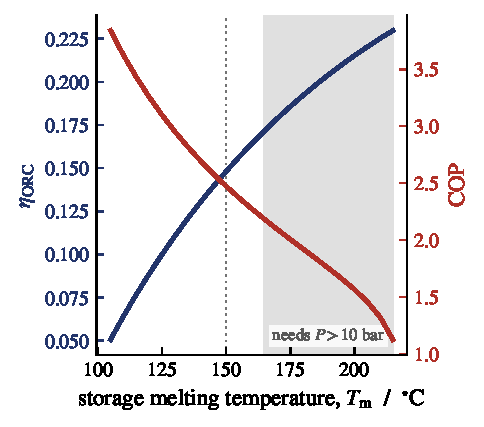
\includegraphics[width=\linewidth]{figures/panels/Tm_a.pdf}
  \caption{}\label{fig:Tm-a}
\end{subfigure}\hfill
\begin{subfigure}[t]{0.48\linewidth}
  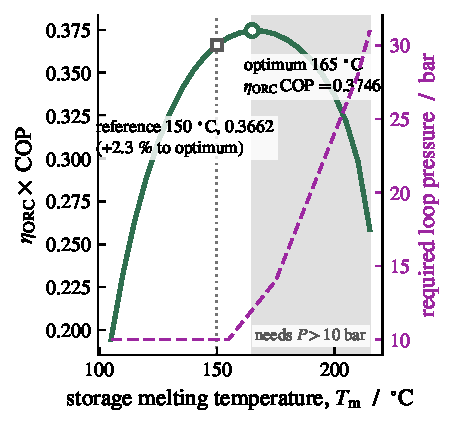
\includegraphics[width=\linewidth]{figures/panels/Tm_b.pdf}
  \caption{}\label{fig:Tm-b}
\end{subfigure}
\\[2.2ex]
\begin{subfigure}[t]{0.48\linewidth}
  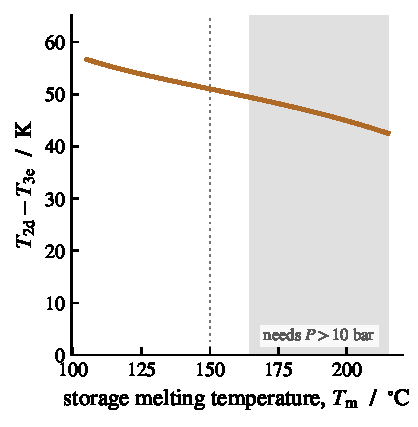
\includegraphics[width=\linewidth]{figures/panels/Tm_c.pdf}
  \caption{}\label{fig:Tm-c}
\end{subfigure}
\caption{Surface cycles against storage temperature. (a) the two machines pull in opposite directions; (b) their product has a shallow maximum at \SI{165}{\celsius}, with the dashed line giving the loop pressure needed to keep the water liquid at the charging inlet; (c) the shortfall between the water arriving from the store and the pinch-limited evaporating temperature, \SIrange{42}{57}{\kelvin} across the whole range, so the interior pinch described in Section~\ref{sec:res-cycles} is a property of the plant and not of the reference case. Shaded: infeasible at the reference loop pressure. Dotted: the reference case.}
\label{fig:Tm}
\end{figure}

\paragraph{Efficiency and capacity optimize in opposite corners}
Figure~\ref{fig:map-cascade} maps the round-trip efficiency, the energy
density per meter of well and the formation loss over the two parameters
that define the cascade. The two objectives do not share an optimum:
$\eta_\mathrm{RTE}$ peaks at $(T_\mathrm{m},\Delta
T_\mathrm{3C,2C})=(\SI{135}{\celsius},\SI{25}{\kelvin})$ at 0.336, while
$e'$ peaks at $(\SI{195}{\celsius},\SI{25}{\kelvin})$ at
\SI{0.482}{\kilo\watt\hour\per\meter}. Efficiency wants a cool store and
capacity wants a hot one, because the loss rises monotonically with
$T_\mathrm{m}$, from \SIrange{5.7}{13.3}{\percent} across the map, while the
latent inventory per meter rises faster. The reference case,
$(\SI{150}{\celsius},\SI{55}{\kelvin})$, sits at neither: moving to the
efficiency optimum gains \SI{12.5}{\percent} of $\eta_\mathrm{RTE}$ and costs
\SI{9}{\percent} of $e'$.

A narrow cascade glide improves \emph{both} objectives at every storage
temperature, with no cell in the map where \SI{55}{\kelvin} beats
\SI{25}{\kelvin}. If the \SI{55}{\kelvin} of the reference is set by a
consideration outside this model --- the number of distinct materials
available, or the grading of the layers --- that should be stated, because
within the model it is pure cost. \chk{confirm whether $\Delta
T_\mathrm{3C,2C}$ is constrained by the PCM selection; if not, the reference
glide should be reduced.}

\begin{figure}[htbp]
\centering
\begin{subfigure}[t]{0.48\linewidth}
  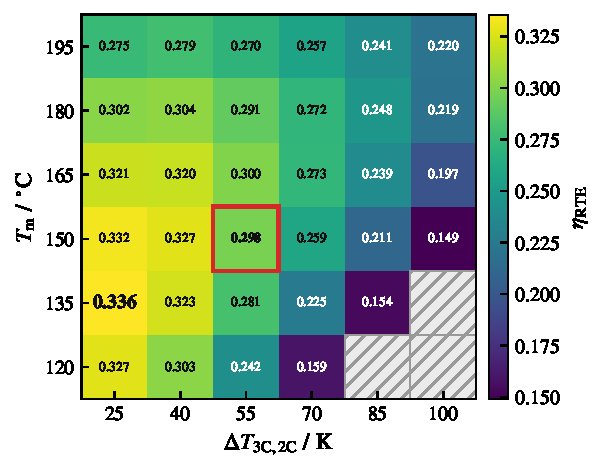
\includegraphics[width=\linewidth]{figures/panels/map_cascade_a.pdf}
  \caption{}\label{fig:map-cascade-a}
\end{subfigure}\hfill
\begin{subfigure}[t]{0.48\linewidth}
  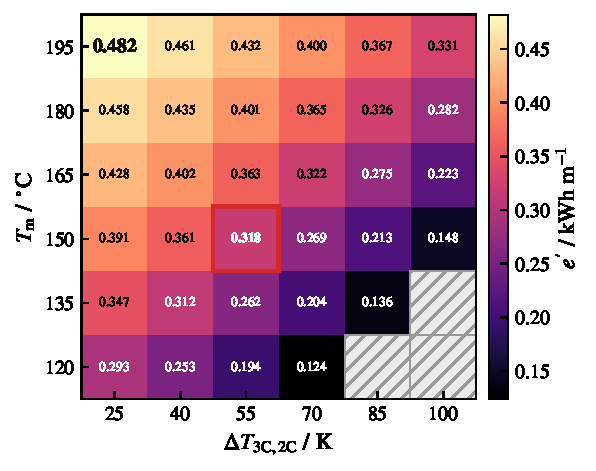
\includegraphics[width=\linewidth]{figures/panels/map_cascade_b.pdf}
  \caption{}\label{fig:map-cascade-b}
\end{subfigure}
\\[2.2ex]
\begin{subfigure}[t]{0.48\linewidth}
  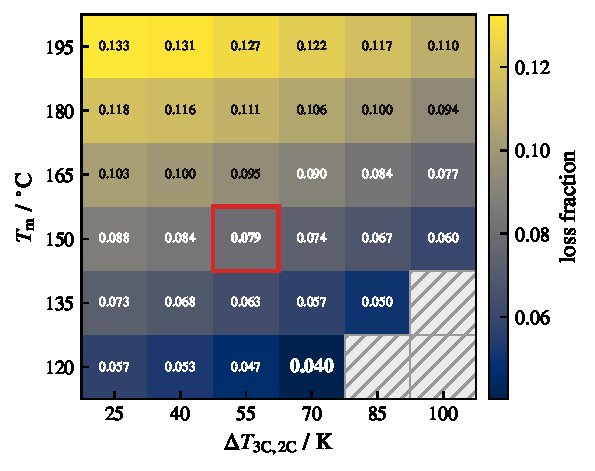
\includegraphics[width=\linewidth]{figures/panels/map_cascade_c.pdf}
  \caption{}\label{fig:map-cascade-c}
\end{subfigure}
\caption{The cascade design space, 36 cyclic-steady-state evaluations: (a) round-trip efficiency, (b) energy density $e'$, (c) formation loss. Above \SI{165}{\celsius} the loop pressure is raised to keep the water liquid, so those rows carry a pressure cost not shown here. In every panel the value in the \textbf{reference-case} cell is set in bold and its cell outlined in red; the value in the \textbf{best} cell of that panel is set in bold at a larger size. Hatched cells are infeasible. Values are printed on the cells because several of these maps are deliberately flat, and flatness cannot be judged from colour alone.}
\label{fig:map-cascade}
\end{figure}

\paragraph{Capacity is set by total bore length, not by how it is divided}
Figure~\ref{fig:map-geometry}(a) and (b) extend to a grid the separability
used in Section~\ref{sec:res-formation}. Over a sixfold range of useful well
length, $e'$ varies by \SIrange{3.4}{3.8}{\percent} \emph{at every layer
count}, and $\eta_\mathrm{RTE}$ by \SIrange{2.4}{3.4}{\percent}, while across
the layer count the same map spans \SI{27.6}{\percent} and
\SI{9.9}{\percent}. Capacity is therefore proportional to total vertical bore
length to within a few percent, and the per-well depth survey that is not
available for THUMS is not required: only the mean enters.

Panel (c) shows that a single fin tube per well is not a design option.
At $\nft=1$ the round-trip efficiency collapses from 0.259 at \SI{1000}{ft}
to 0.077 at \SI{6000}{ft} on pumping alone, because the whole flow passes
through one tube. From $\nft=3$ the map is flat in both directions and the
reference sits comfortably inside it, with $\nft=4$ marginally better
(0.298 against 0.293).

\begin{figure}[htbp]
\centering
\begin{subfigure}[t]{0.48\linewidth}
  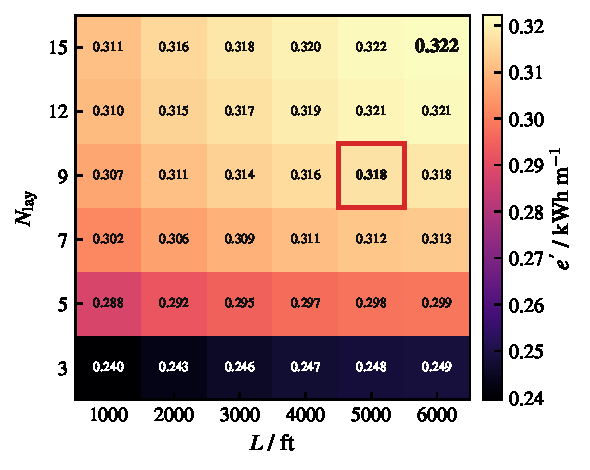
\includegraphics[width=\linewidth]{figures/panels/map_geom_a.pdf}
  \caption{}\label{fig:map-geometry-a}
\end{subfigure}\hfill
\begin{subfigure}[t]{0.48\linewidth}
  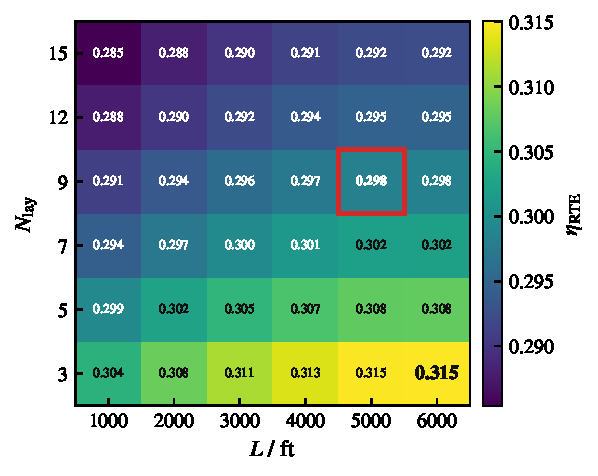
\includegraphics[width=\linewidth]{figures/panels/map_geom_b.pdf}
  \caption{}\label{fig:map-geometry-b}
\end{subfigure}
\\[2.2ex]
\begin{subfigure}[t]{0.48\linewidth}
  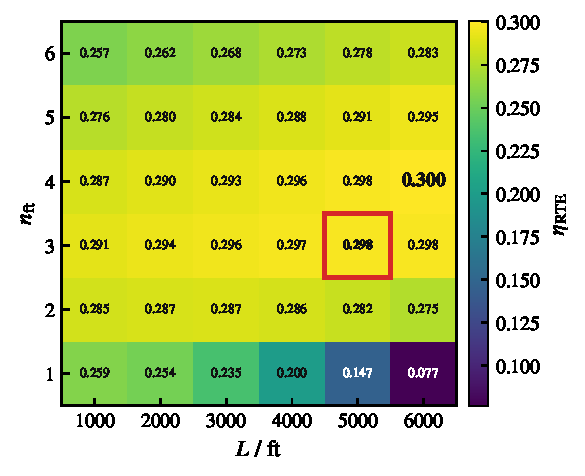
\includegraphics[width=\linewidth]{figures/panels/map_geom_c.pdf}
  \caption{}\label{fig:map-geometry-c}
\end{subfigure}
\caption{Geometry maps: (a) $e'$ and (b) $\eta_\mathrm{RTE}$ over well length and layer count, (c) $\eta_\mathrm{RTE}$ over well length and fin-tube count. The near-constancy of (a) and (b) along the horizontal is the separability result, not a rendering artifact. In every panel the value in the \textbf{reference-case} cell is set in bold and its cell outlined in red; the value in the \textbf{best} cell of that panel is set in bold at a larger size. Hatched cells are infeasible. Values are printed on the cells because several of these maps are deliberately flat, and flatness cannot be judged from colour alone.}
\label{fig:map-geometry}
\end{figure}

\paragraph{The apparent dependence on the number of layers is the cascade
span} $\Nlay$ cannot be varied on its own. The span of the melting
temperatures is one layer width short of the grading parameter,
$\mathrm{span}=\Delta T_\mathrm{cascade}(\Nlay-1)/\Nlay$, so sweeping
$\Nlay$ at fixed $\Delta T_\mathrm{3C,2C}$ widens the span as well and the
two effects are confounded. Done that way, $\eta_\mathrm{RTE}$ falls
monotonically by \SI{7.5}{\percent} from $\Nlay=3$ to $\Nlay=15$ and the
result looks like a recommendation for few layers.

Holding the span fixed at the reference \SI{48.9}{\kelvin} by setting
$\Delta T_\mathrm{cascade}=\mathrm{span}_0\,\Nlay/(\Nlay-1)$ removes the
trend entirely: above $\Nlay=7$ the round-trip efficiency is constant to
\SI{0.19}{\percent} and $e'$ to \SI{0.8}{\percent}
(Figure~\ref{fig:nlay}). The layer count is converged at the reference
value of 9, and the apparent benefit of few layers was the narrower span
those cases happened to carry. Only the low-$\Nlay$ end retains a real
dependence, where there are too few layers to grade the store at all.

\begin{figure}[htbp]
\centering
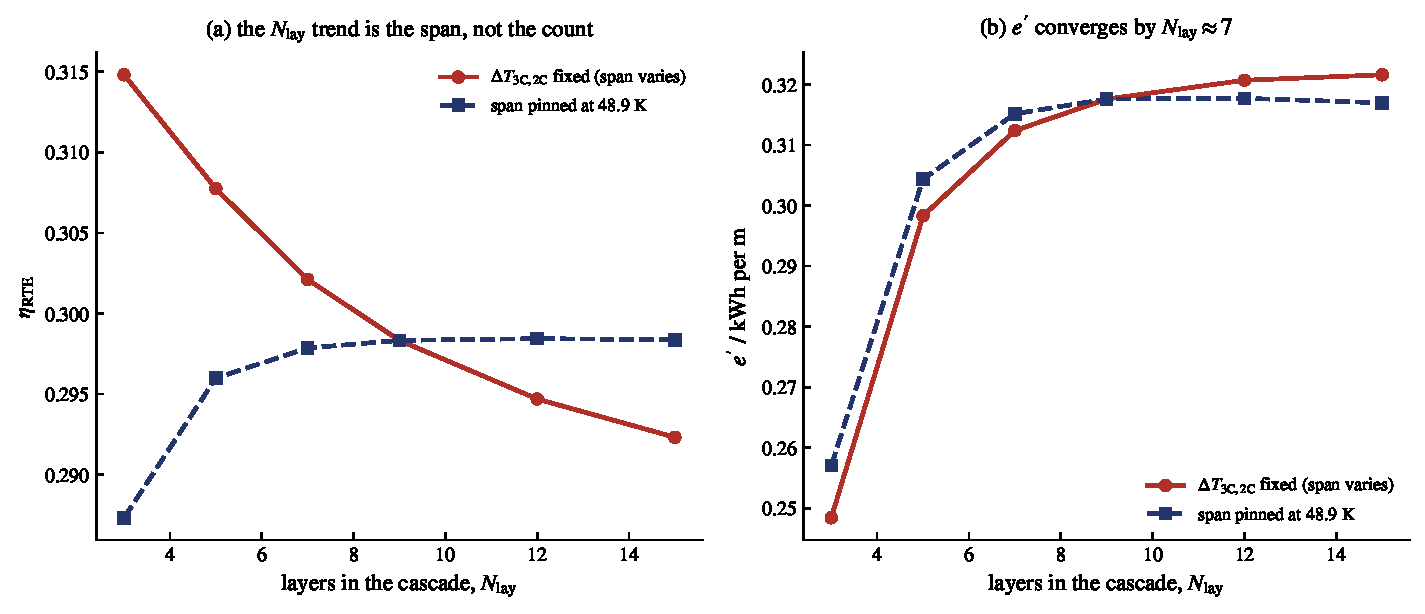
\includegraphics[width=0.82\linewidth]{figures/BOREAS_Nlay_confound.pdf}
\caption{Breaking the confound between the layer count and the cascade span.
Red: $\Delta T_\mathrm{3C,2C}$ held fixed, so the span varies with $\Nlay$.
Blue: the span pinned at \SI{48.9}{\kelvin}. The monotonic trend in the first
is the span, not the layer count.}
\label{fig:nlay}
\end{figure}

\paragraph{Shielding depends on divergence more than on number}
Figure~\ref{fig:map-field} maps the loss over the well count and the fan
half-angle at the realistic rows packing, and over the geothermal gradient
and the storage length. The first panel makes the conclusion of
Section~\ref{sec:res-formation} a surface rather than two rows of a table:
the loss falls from \SI{18.6}{\percent} to \SI{7.9}{\percent} as the count
rises from 10 to 1000 at $\theta=0$, but rises to \SIrange{22}{68}{\percent}
as soon as the wells diverge at all. Beyond that the two variables trade:
at 3000 wells the loss still trebles between \SI{15}{\degree} and
\SI{75}{\degree}, while at 10 wells it is flat at about
\SI{69}{\percent} because those wells are effectively isolated whatever the
angle. Divergence, not number, is the dominant variable once the packing is
realistic, and the number only buys shielding while the wells stay close. \chk{at large $\theta$ the rows description is itself
questionable: $P(z)=P_0R_f(z)/R_0$ scales a row perimeter with the fan
radius, and wells spread over 6500 acres are not in rows at depth. The rows
and disc results should be read as bounding the arrangement, not as
alternatives one of which is correct.}

The third panel shows that depth and gradient reinforce one another rather
than oppose. Loss falls with storage length at every gradient, because a
fixed perimeter is shared by more storage as the wells deepen, and it falls
with the gradient as well, because hotter rock reduces the driving difference
against a \SI{150}{\celsius} store. The two interact strongly: at
\SI{1000}{ft} the gradient is almost irrelevant
(\SIrange{10.4}{11.2}{\percent} from \SIrange{85}{35}{\kelvin\per\kilo\metre}),
whereas at \SI{6000}{ft} it changes the loss threefold
(\SIrange{3.2}{9.2}{\percent}), since only a deep well reaches the rock the
gradient has warmed. For Wilmington, where the gradient is high, this is
favourable and it argues for taking the storage as deep as the vertical
section allows --- subject to the \chk{} on the true vertical depth in
Section~\ref{sec:res-formation}.

\begin{figure}[htbp]
\centering
\begin{subfigure}[t]{0.48\linewidth}
  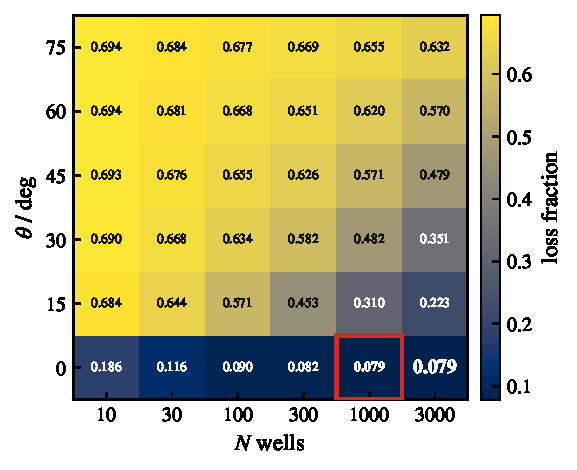
\includegraphics[width=\linewidth]{figures/panels/map_field_a.pdf}
  \caption{}\label{fig:map-field-a}
\end{subfigure}\hfill
\begin{subfigure}[t]{0.48\linewidth}
  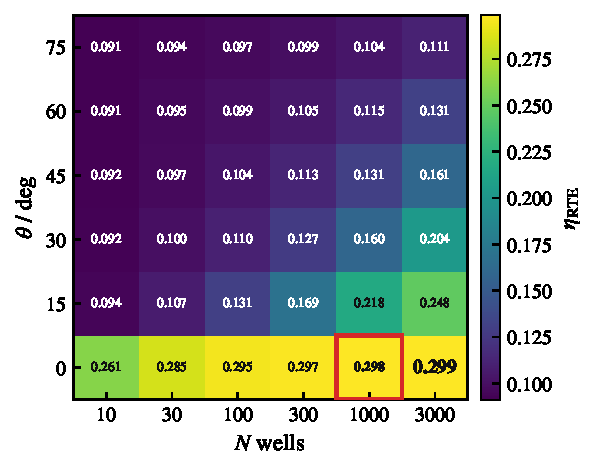
\includegraphics[width=\linewidth]{figures/panels/map_field_b.pdf}
  \caption{}\label{fig:map-field-b}
\end{subfigure}
\\[2.2ex]
\begin{subfigure}[t]{0.48\linewidth}
  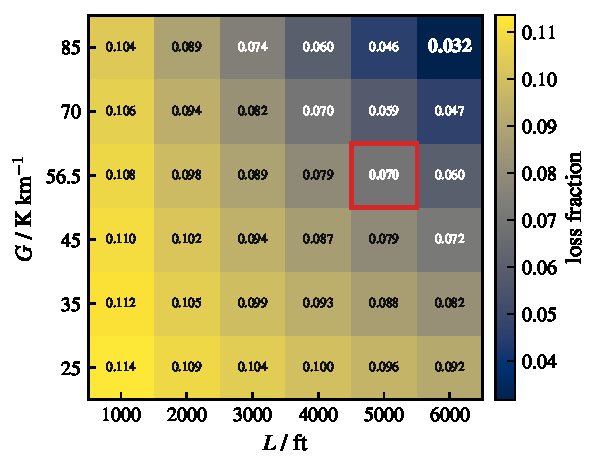
\includegraphics[width=\linewidth]{figures/panels/map_field_c.pdf}
  \caption{}\label{fig:map-field-c}
\end{subfigure}
\caption{Field maps at the rows packing on four islands: (a) formation loss and (b) $\eta_\mathrm{RTE}$ over well count and fan half-angle, (c) formation loss over well length and geothermal gradient. Panels (a) and (b) use the realistic packing throughout, so their \SI{45}{\degree} column is \emph{not} comparable with the disc-packing fan rows of Table~\ref{tab:formation}. In every panel the value in the \textbf{reference-case} cell is set in bold and its cell outlined in red; the value in the \textbf{best} cell of that panel is set in bold at a larger size. Hatched cells are infeasible. Values are printed on the cells because several of these maps are deliberately flat, and flatness cannot be judged from colour alone.}
\label{fig:map-field}
\end{figure}
